\section{Internet of things}
%Write an introduction to this and choose ONE quote.
Cluster of European research projects regarding the Internet of Things:
\begin{quote}
    'Things' are active participants in business, information and social processes where they are enabled to interact and communicate among themselves and with the environment by exchanging data and information sensed about the environment while reacting autonomously to real/physical world events and influencing it by running processes that trigger actions and create services with or without direct human intervention.\cite{Gubbi2013}
%Fix correct quote on this!
\end{quote} 

Gubbi et al. define the Internet of Things as:
\begin{quote}
    Interconnection of sensing and actuating devices providing the ability to share information across platforms through a unified framework, developing a common operating picture for enabling innovative applications. 
    Achieved by seamless large scale sensing, data analytics, and information representation using cutting edge ubiquitous sensing and cloud computing.\cite{Gubbi2013}
\end{quote}

\section{Industry 4.0}
%Industry 4.0 definition.
Lasi argues that the term industry 4.0 was coined beforehand as a planned fourth industrial revolution.\cite{Lasi2014}
The use of internet of things devices, IoT devices from now on, and cyber-physical systems, CPS from now on is what defines the fourth industrial revolution Vadiya means.\cite{Vaidya2018}
See figure x for a short historic overview of previous industrial revolutions.   
\begin{figure}
    \centering
    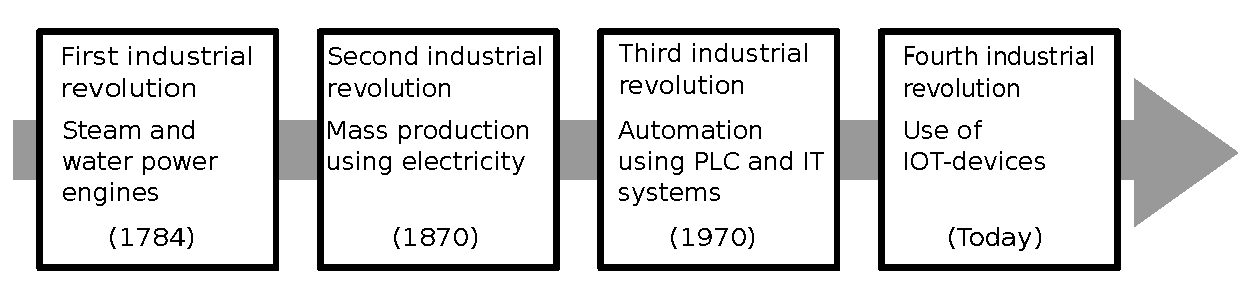
\includegraphics[width=\textwidth]{Pictures/Industrial_revolution.pdf} 
    \caption{Historic overview of previous industrial revolutions}
    \label{Indutrial revolutions}
\end{figure}

According to Vaidya, industry 4.0 promotes connecting sensors and devices to the internet and other sensors or devices.\cite{Vaidya2018} 

%Intelligent sensors.
Hozdić states that a sensor is a device capable of providing an appropriate output in response to a measured value.
One key feature of an intelligent sensor is that it increases information processing, and it processes the information at a logical level, Hozdić argues.
An Intelligent sensor  is capable of executing actions based on the measured value in contrast to regular sensors, making them easier to set up and use means Hozdić.\cite{Hozdic2015} 

%Cyber Physical Systems (CPS).
Hozdić defines a cyber-physical system, CPS, as a new generation of a system that integrates physical and computer abilities.
A cyber-physical system consists of two parts, one cybernetic and one physical.
The cybernetic aspect of the system is a summation of logic and sensor units. In contrast, the physical part of the system is the summation of the actuator units, Hozdić adds.
Xu et al. state that cyber-physical systems are a vital part of Industry 4.0. In contrast to the simple embedded systems of today will be exceeded due to advances in CPS that enable enhanced capability, scalability, adaptability, resiliency, safety, usability, and security.\cite{Xu2018}
Hozdić argues that the CPS can share and receive information from intelligent sensors connected to digital networks, enabling and forming an internet of things.\cite{Hozdic2015}
 
\section{Arrowhead framework}
%Local cloud.
Delsing defines a local cloud as a self-contained network with at least the three mandatory systems deployed, more on those in a later paragraph. 
Delsing et al. also argue that the three mandatory core systems running a local cloud also need at least one application system deployed.\cite{Delsing2017}

%Service and systems.
To further understand what the Eclipse Arrowhead framework aims to accomplish, introducing the terms services and systems is necessary.
Delsing et al. define a system as providing or consuming a service.
Furthermore, Delsing et al. define a service as conveying information between a provider and a consumer.\cite{Delsing2017}

%Mandatory core systems.
The Eclipse Arrowhead framework, Arrowhead from now on, consists of three mandatory core systems according to Delsing et. al.
To fully operate a local cloud as defined in the previous section it must, according to Delsing, contain:
\begin{itemize}
    \item Service registry system.
    \item Authorization system. 
    \item Orchestration system.\cite{Delsing2017}
\end{itemize} 

\begin{figure}[H]
    \centering
    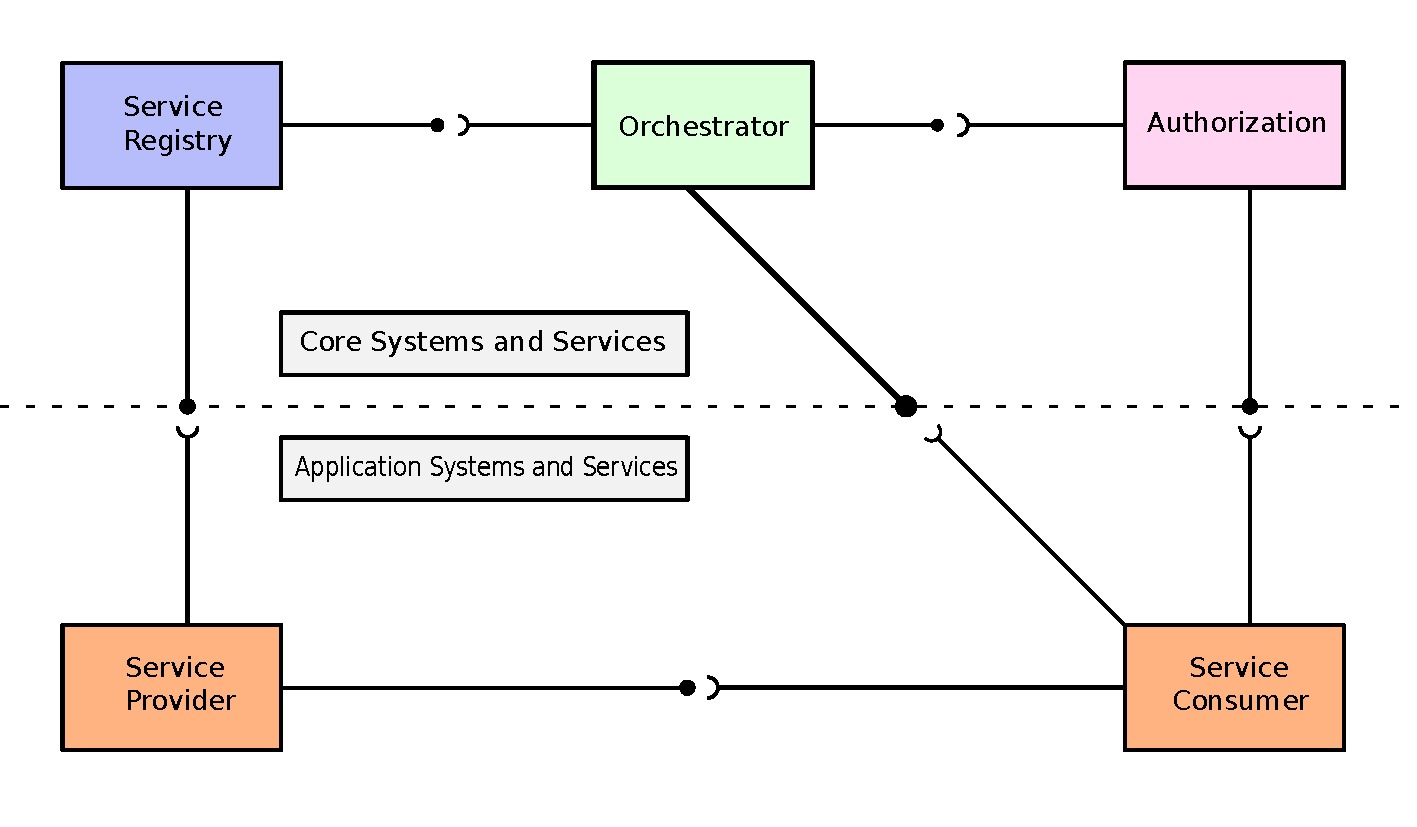
\includegraphics[width=\textwidth]{Pictures/ah.pdf} 
    \caption{The core systems of the Eclipse Arrowhead framework}
    \label{diagram arrowhead}
\end{figure}
The dynamics between the consumer and provider system will follow in the theory section.
\section{Amazon Web Services}
%Intro
According to the Amazon webpage, the AWS IoT Core connectivity services consist of the device gateway, message broker, and rules engine.

%Deivce gateway
The device gateway enables devices to securely, via X.509 certificates, and efficiently communicate with AWS IoT Amazon.

%Message broker
Amazon states that the message broker provides a secure way for devices and AWS IoT applications to publish or receive, subscribe as known in MQTT, messages from each other.
The message broker also distributes device data to devices that have subscribed to it and to other AWS IoT Core services, such as the rules engine Amazon adds. 

%Rules engine
The Rules engine connects data from the message broker to other AWS services, such as Amazon Simple Storage Service (Amazon S3), Amazon DynamoDB, and AWS Lambda, according to Amazon.\cite{AWS2021}

\begin{figure}[H]
    \centering
    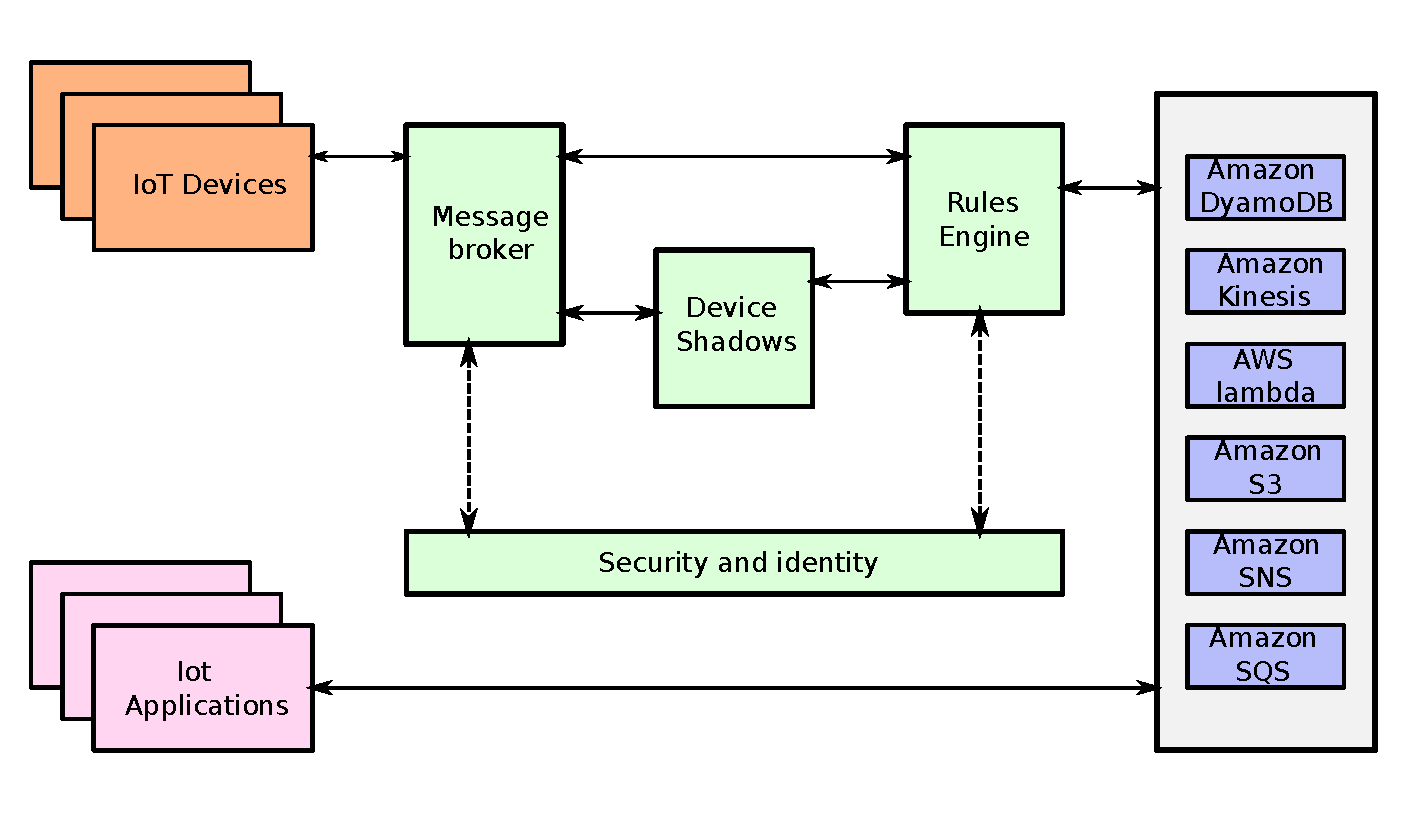
\includegraphics[width=\textwidth]{Pictures/aws.pdf} 
    \caption{The core systems of the Amazon Web Services}
    \label{diagram AWS}
\end{figure}

\section{Security}
%Introduction.
Meneghello et al. argue that the increasing number of IoT devices and the pervasive nature of new smart home or healthcare devices can pose a real threat to the users' integrity.
Meneghello et al. define sensitive information as a video recording of the user's home, location, access to buildings, health monitoring, and industrial processes.\cite{Meneghello2019}

%Secruity challenges.
Meneghello et al. divide the security requirements of an IoT system into three different operational levels: the information, access, and functional level.
The information level should guarantee the preservation of the system's integrity, anonymity, confidentiality, and privacy. 
To maintain integrity, no alteration of the messages can occur during transmission. The identity of the data source and the clients' private information remains hidden. Third parties cannot read that data, Meneghello et al. argue.
The access level guarantees that only legitimate users can access the network and the devices associated with that network. 
It also guarantees that users within the network only use resources they can use, Meneghello et al. state.
The functional level should guarantee the continued functionality of a network even in the case of malfunction or a malicious attack, Meneghello et al. add.\cite{Meneghello2019}

%Pricacy.
Zhang also argues that privacy is a big concern with IoT devices and suggests two solutions data collection policy and data anonymization.
A policy that describes how data collected from the devices would restrict data flow, ensuring privacy preservation, Zhang states.
Data anonymization means that private information sent by the IoT devices is either encrypted or conceals the relation of the data and its owner according to Zhang.\cite{Zhang2014}

%Encryption.
Meneghello et al. argue that one of the main aspects of security within IoT is to ensure that the data sent is the data received and that the data has not been tampered with or read during transmission.
The most critical operation to guarantee is encryption, which converts the message sent in plain text to an encrypted message only readable with a decryption key, Meneghello et al. state.
Meneghello et al. state that there are two mechanisms for encryption, symmetric and asymmetric.
Symmetric encryption uses the same key for encryption and decryption, sharing it with both the sender and receiver.
On the other hand, asymmetric encryption only shares the public key, and the sender and receiver have their private keys Meneghello et al. means.\cite{Meneghello2019}

%End-to-End encryption.
Hassija et al. state the importance of end-to-end encryption and its challenges for IoT systems.
End-to-end encryption is required to ensure the confidentiality of the data. The application should not let anyone except the intended recipient read the messages sent Hassija adds.\cite{Hassija2019}

%Authentification.
Noor, Meneghello, and Zhang state the importance of authentification in IoT systems.\cite{Noor2019,Meneghello2019,Zhang2014} 
Noor adds that 60\% of all IoT systems use authentification to grant access to the user.\cite{Noor2019}  
Zhang argues that public key cryptosystem provides more security than symmetric encryption schemes but has the drawback of having high computational overhead.\cite{Zhang2014} 

%Lightweight cryptography.
Noor argues that conventional cryptographic primitive is unsuitable for IoT devices due to their lack of computational power and limited battery life and memory capacity.\cite{Noor2019}
With IoT devices lacking capabilities as background Noor, Meneghello, and Zhang all agree that a push for lightweight cryptography is required to ensure the security of these devices.\cite {Noor2019,Meneghello2019,Zhang2014} 

\section{Communication} 
%MQTT
MQTT, Message Queue Telemetry Transport, is a lightweight messaging invented by IBM suitable for IoT according to Wukkadada.\cite{Wukkadada2018} 
MQTT is a publish/subscribe protocol that requires a minimal footprint and bandwidth to connect an IoT device according to HIVEMQ.\cite{MQTT2021}
MQTT consists of an MQTT broker and MQTT clients, where the broker is responsible for sending messages between the sender and its recipients.\cite{Wukkadada2018}
On the other hand, a client publishes a message to the broker that other clients can subscribe to HIVEMQ add.\cite{MQTT2021}

%HTTP/HTTPS
HTTP, HyperText Transfer Protocol, is a request/response protocol consisting of clients and servers that communicate by exchanging individual messages. 
The clients are responsible for the requests, and the servers are responsible for the response Mozilla developer network clarifies. \cite{HTTP2021} 
In contrast to the lightweight MQTT protocol with low overhead and bandwidth, HTTP can cause serious bandwidth issues, Wukkadada adds. \cite{Wukkadada2018}
The most significant benefits to using HTTP are that it supports the RESTful Web architecture and a globally accepted web messaging standard Naik suggests. \cite{Naik2017} 

%Comparisson 
Naik argues that HTTP exceeds MQTT in message size, message overload, power consumption, resource requirements, bandwidth, and latency. 
All things that are considered adverse for a protocol.
On the other hand, HTTP exceeds MQTT in interoperability, standardization, security, and provisioning, Naik adds.\cite{Naik2017}
All things that are considered positive for a protocol.
Shariatzadeh argues that that HTTP may be expansive for many IoT devices, but it can be beneficial due to the interoperability since initially developed for the web.\cite{Shariatzadeh2016}
Wukkadada also points out the lower power consumption of the MQTT protocol but adds that the more lengthy HTTP protocol can be easier for developers to understand.
Wukkada drives home the point of choosing MQTT for IoT devices.\cite{Wukkadada2018}